\appendix


\chapter{2D Benchmark Phase Portraits}
\label{app:benchmark-portraits}

Phase portraits of the four 2D benchmark systems introduced in
Chapter~\ref{chap:benchmarks}. In each panel the faint streamlines trace the
\emph{expected} one-step drift $\expe_w[f(x,w)] - x$ --- estimated by Monte-Carlo,
so they are valid for additive, switched and state-dependent noise alike --- while
the coloured curves are stochastic sample trajectories rolled out from random
starts inside the domain (dark to light with elapsed time). The domain boundary is
drawn in black and the equilibrium region as a red dashed circle.

\begin{figure}[htbp]
\centering
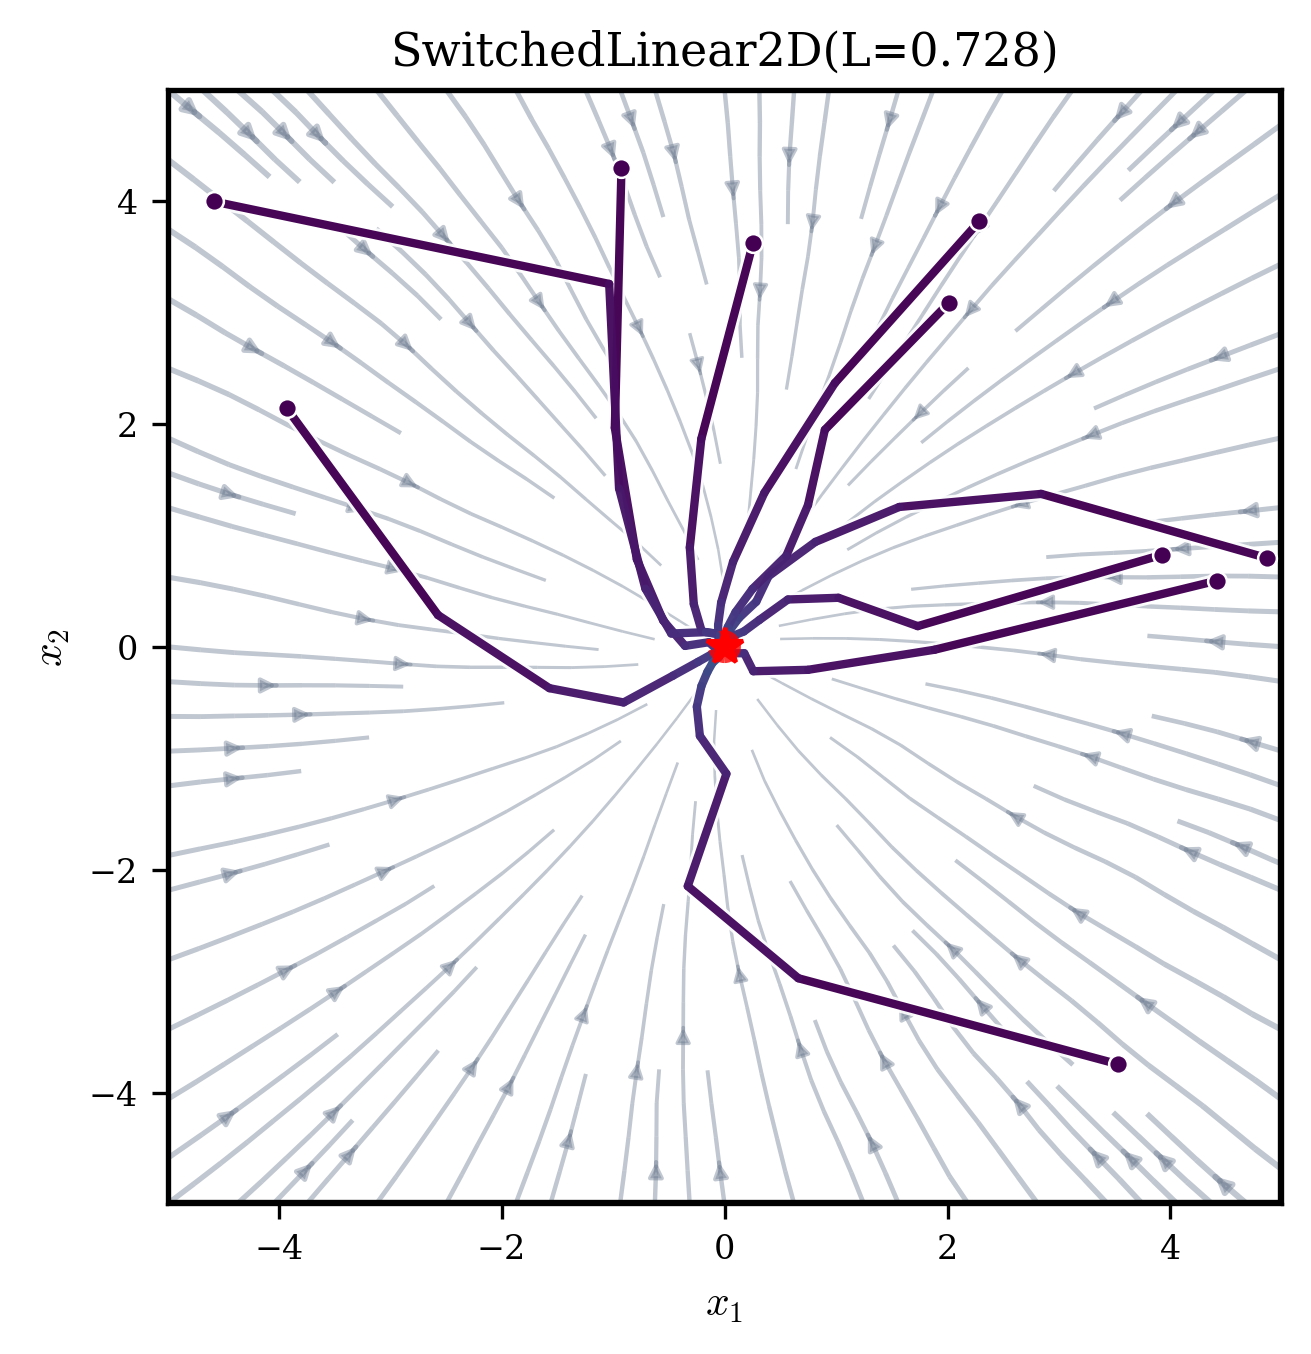
\includegraphics[width=0.55\linewidth]{Figures/linear2D_phase.png}
\caption{$\mathrm{LinSwitch}$ (Section~\ref{sec:bench-switched}): the randomly
switched linear system. Both switching modes are $L_1$-contractive, so every
trajectory collapses to the origin irrespective of the switching sequence.}
\label{fig:phase-linswitch}
\end{figure}

\begin{figure}[htbp]
\centering
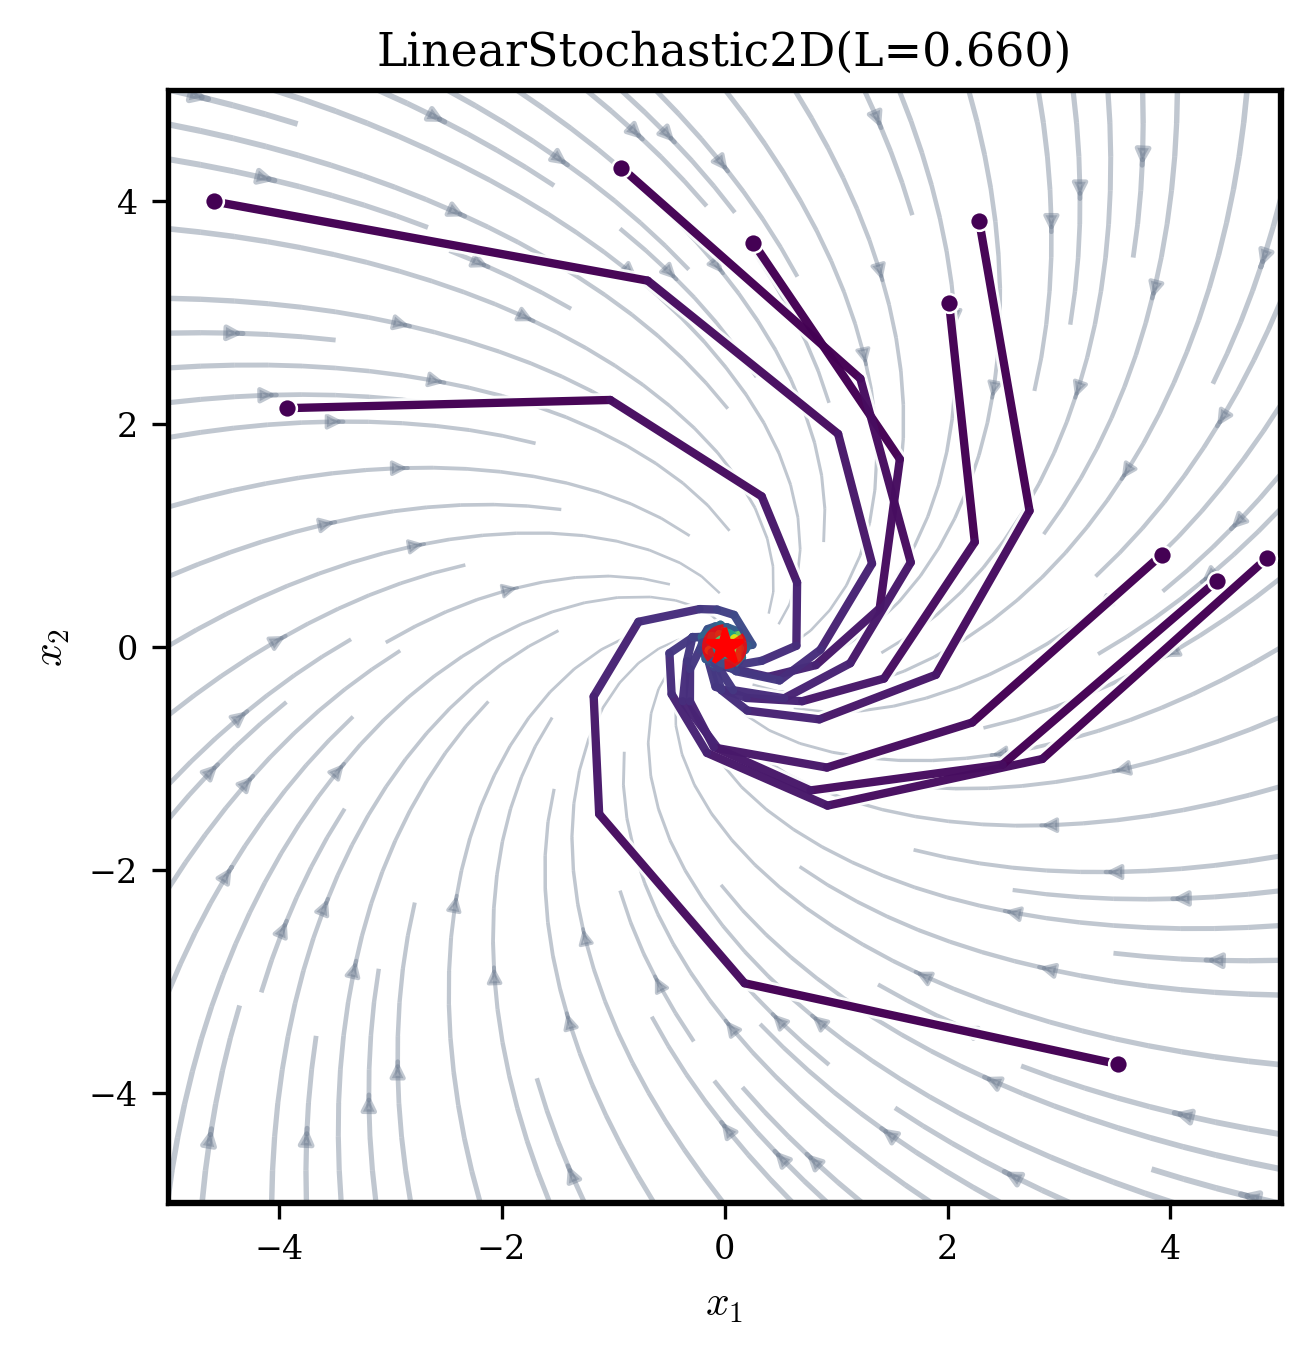
\includegraphics[width=0.55\linewidth]{Figures/linstoch2D_phase.png}
\caption{$\mathrm{LinStoch}$ (Section~\ref{sec:bench-linstoch}): the additive-noise
linear system. The Schur-stable drift spirals trajectories inward until the noise
floor halts them in a neighbourhood of the origin --- the equilibrium ball the
certificate must enclose.}
\label{fig:phase-linstoch}
\end{figure}

\begin{figure}[htbp]
\centering
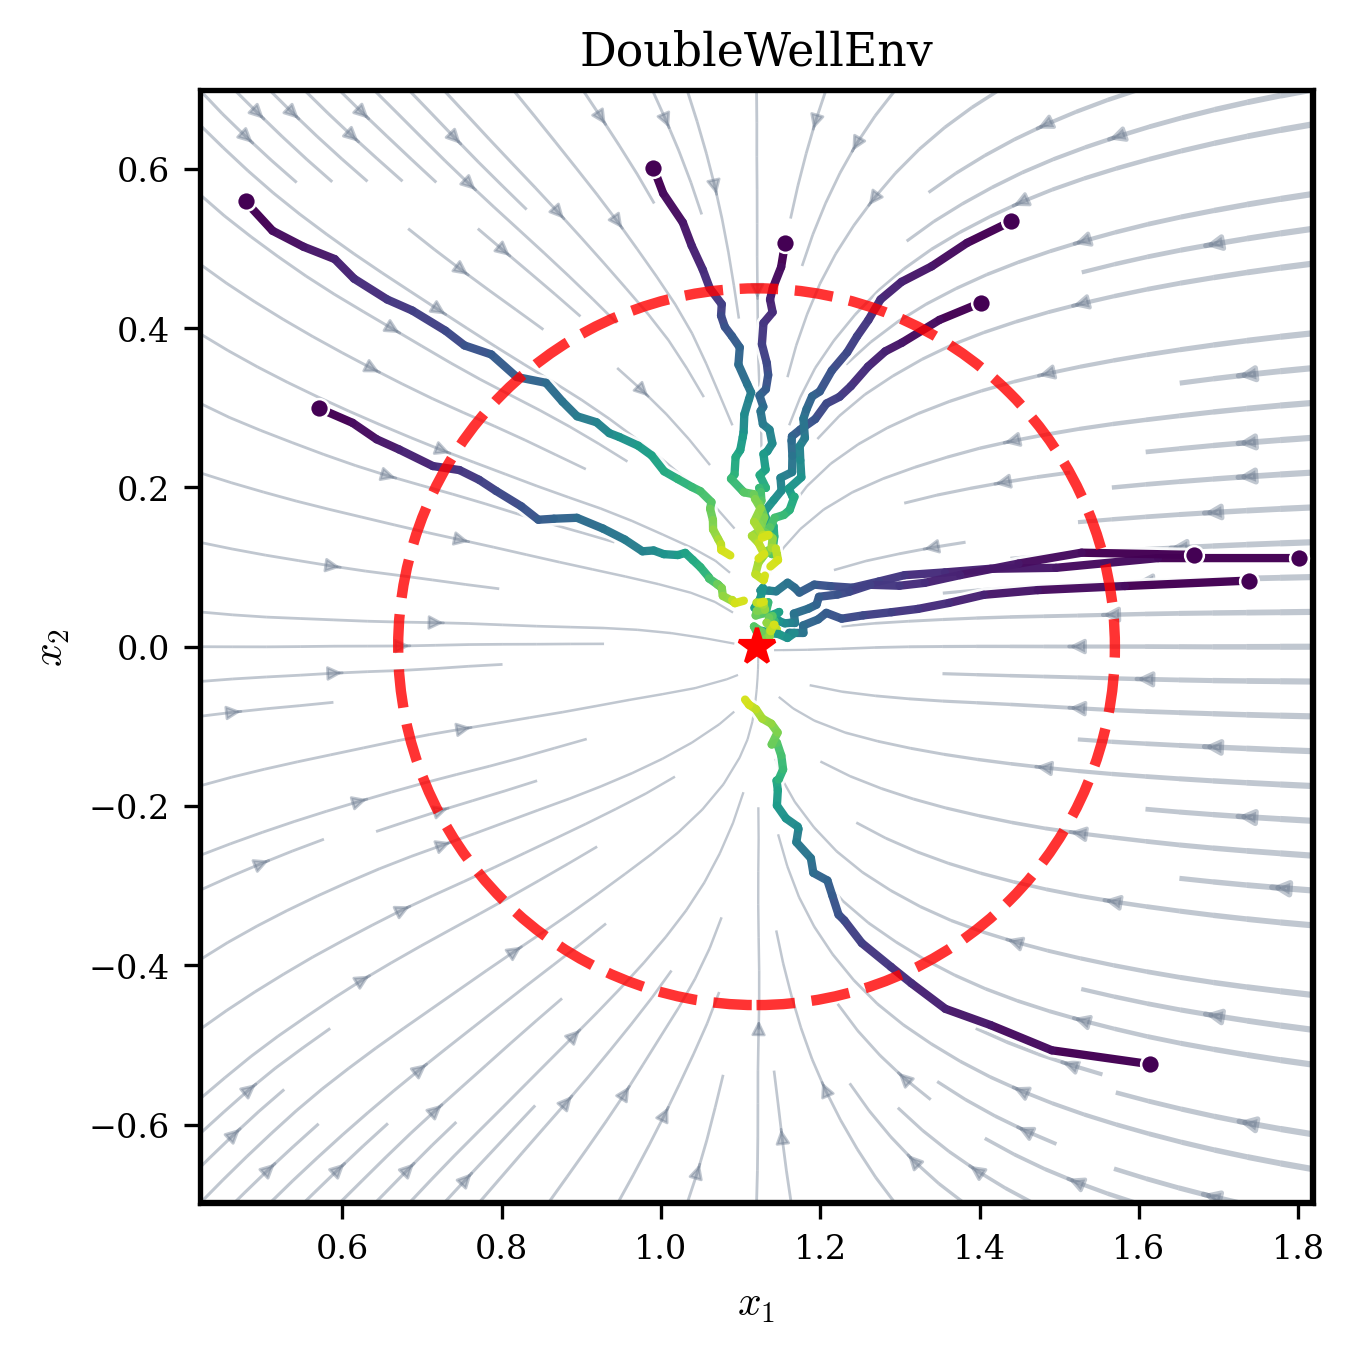
\includegraphics[width=0.55\linewidth]{Figures/doublewell_phase.png}
\caption{$\mathrm{DoubleWell}$ (Section~\ref{sec:bench-doublewell}): the tilted
stochastic gradient flow, shown zoomed onto its true attractor at $\approx(1,0)$
--- the off-origin equilibrium that sets this system apart from the others.}
\label{fig:phase-doublewell}
\end{figure}

\begin{figure}[htbp]
\centering
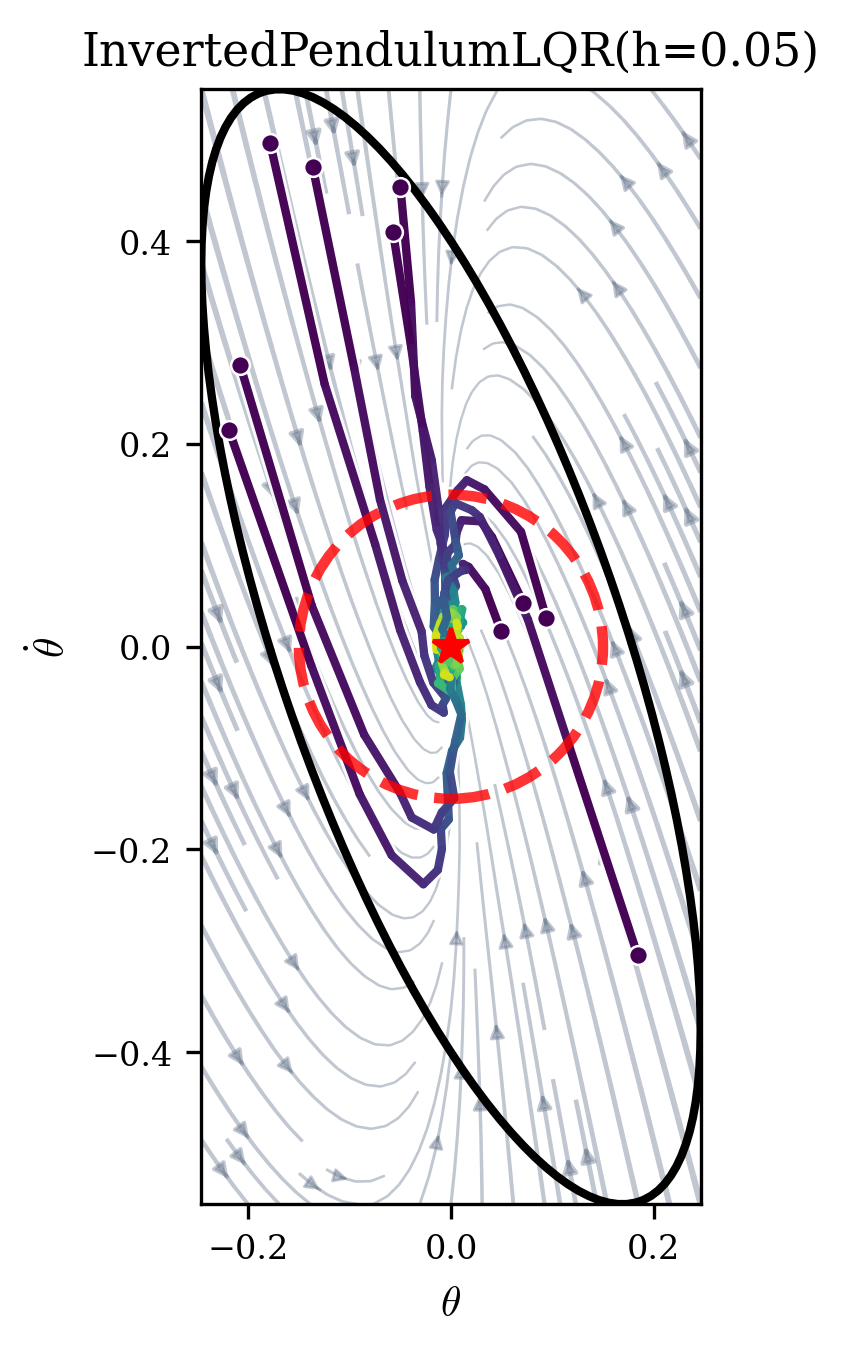
\includegraphics[width=0.36\linewidth]{Figures/pendulum_lqr_phase.png}
\caption{$\mathrm{Pendulum}$ (Section~\ref{sec:bench-pendulum-lqr}): the
LQR-controlled inverted pendulum in the $(\theta,\dot\theta)$ plane. The closed
loop is Schur-stable but non-normal, so the forward-invariant domain is the
Lyapunov sublevel ellipsoid (black) rather than a box; trajectories spiral into
the upright equilibrium.}
\label{fig:phase-pendulum}
\end{figure}


\chapter{Examples of Refuter Search Patterns}

This appendix supplements the refuter benchmark of Section~\ref{sec:bbob} with a
qualitative view of how each method spends its evaluation budget.
Figure~\ref{fig:refuter-patterns} overlays the sampled points of every refuter on
the five BBOB landscapes, at the same fixed budget, making visible the difference
between uninformed search and the informed methods that concentrate around
promising basins.

\begin{figure}[htbp]
\centering
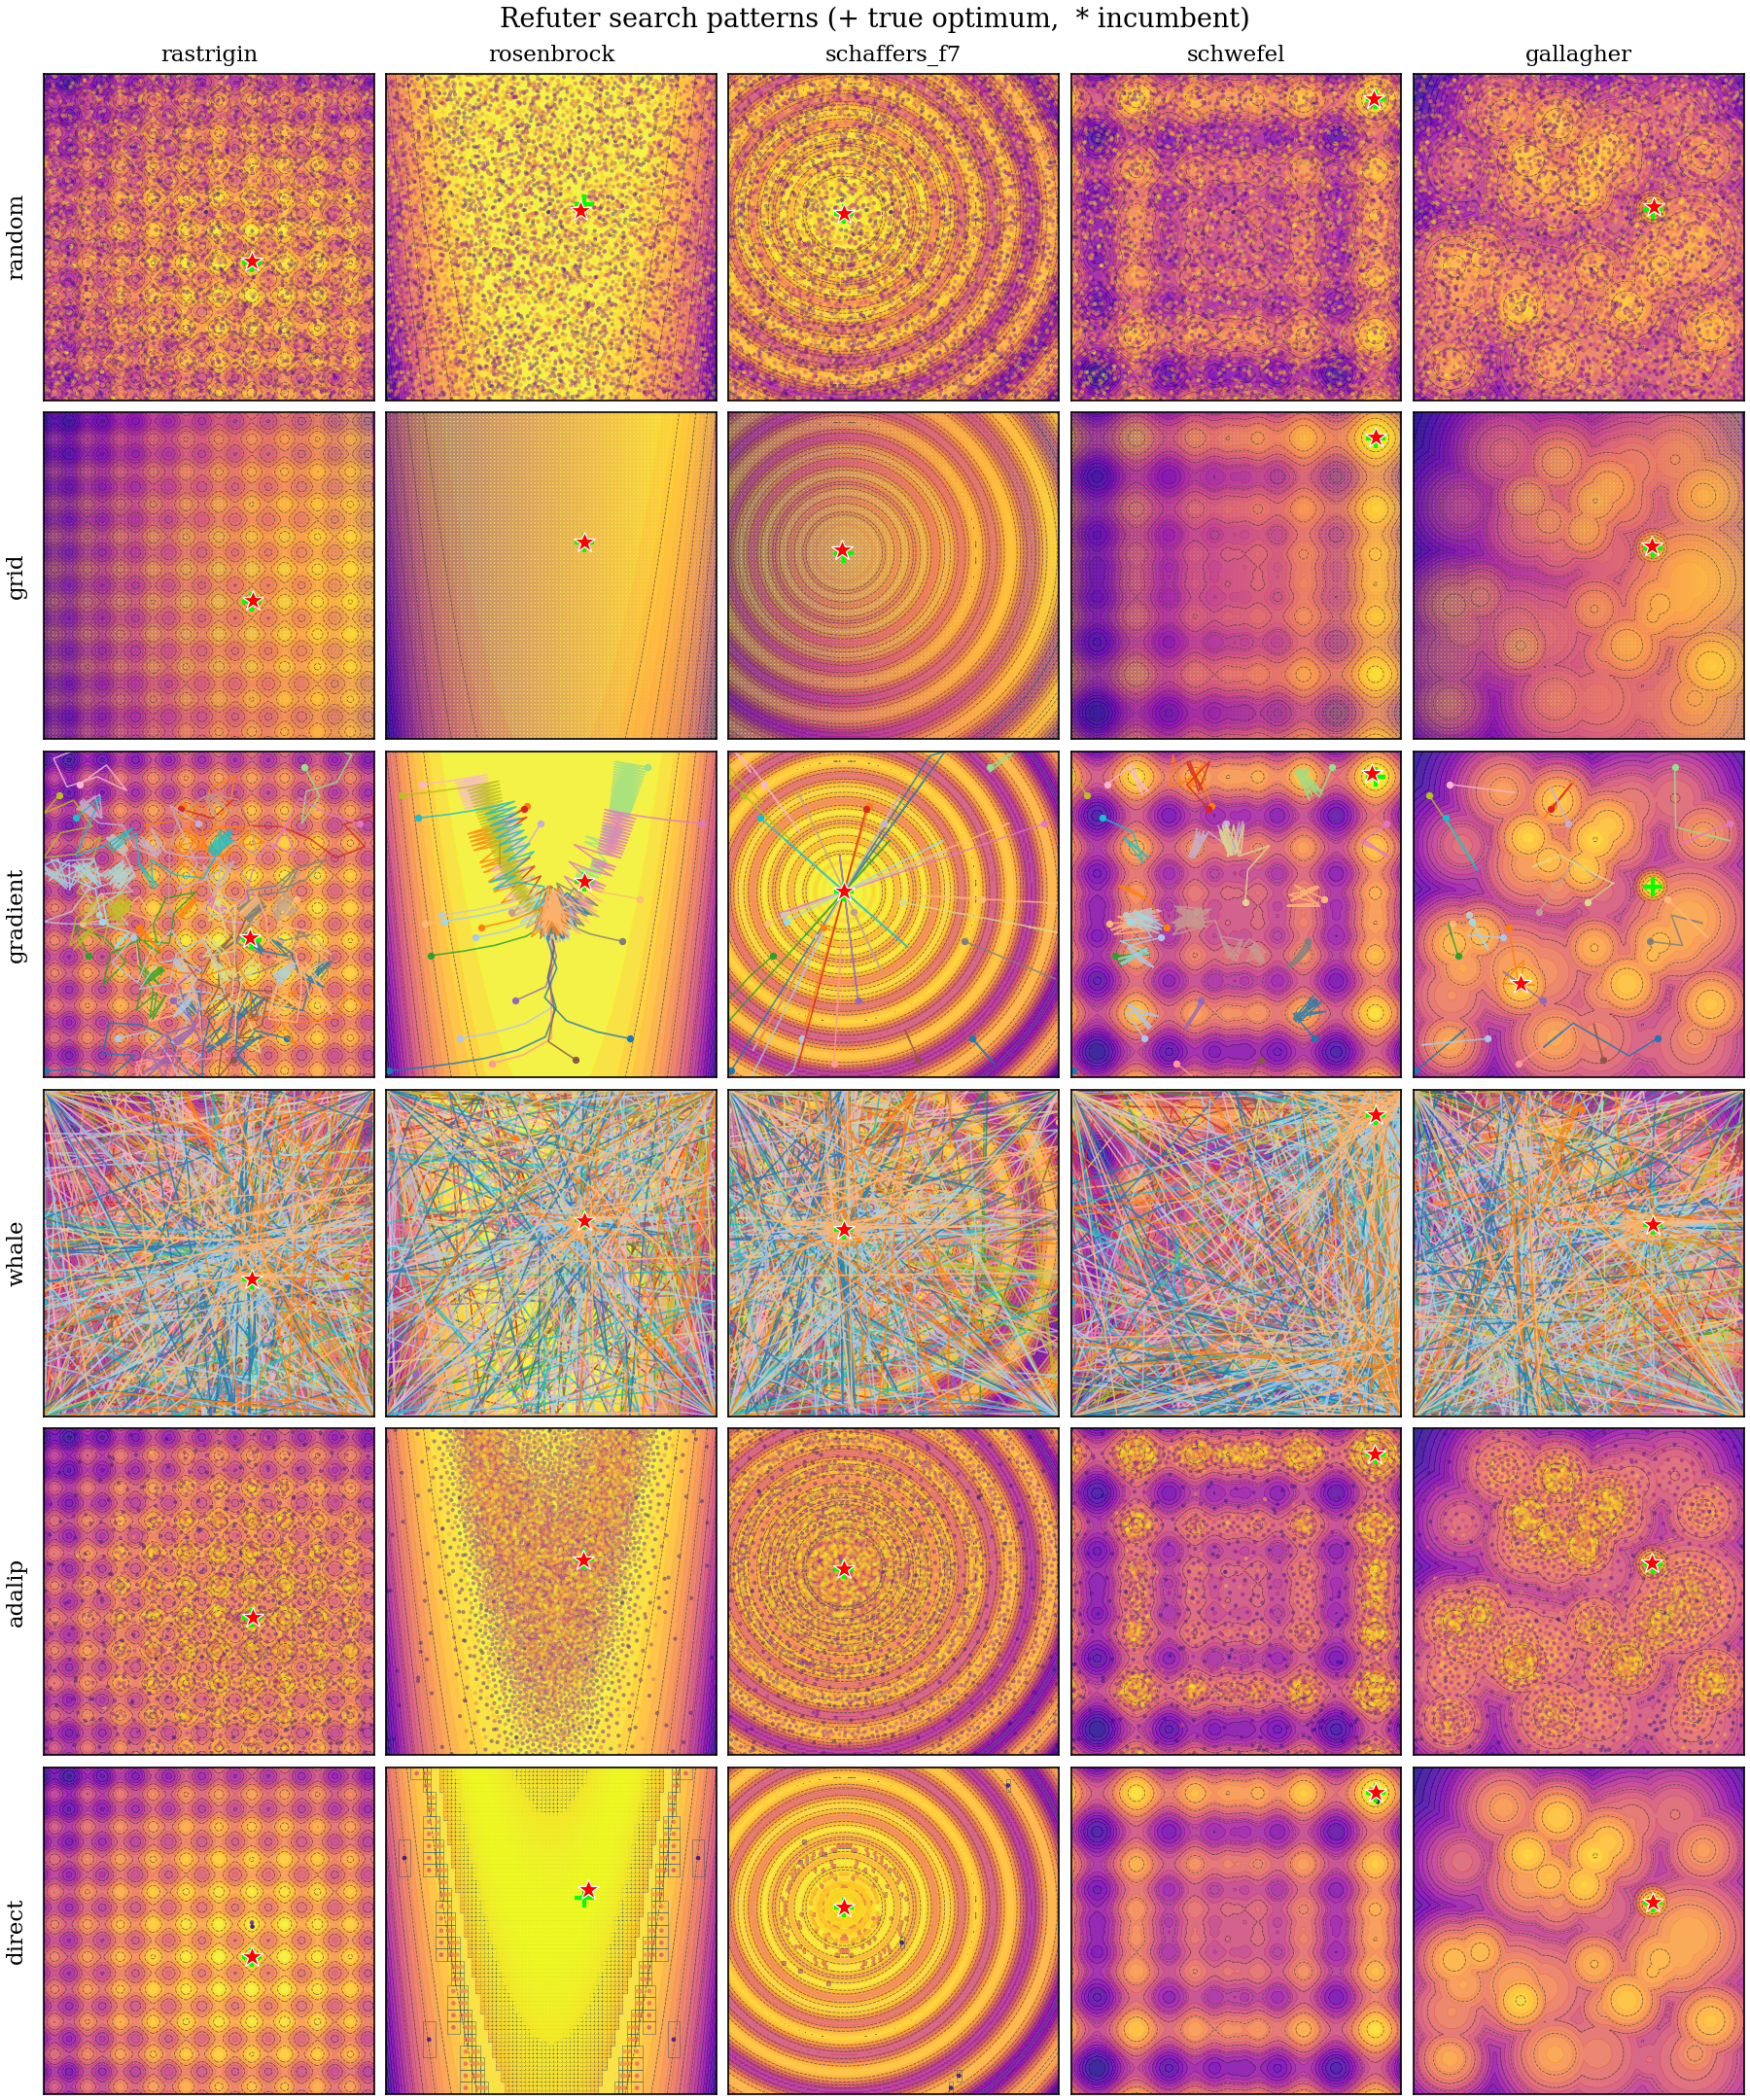
\includegraphics[width=\linewidth]{Figures/refuter_search_patterns.png}
\caption{Evaluation patterns of each refuter over a BBOB landscape at a fixed
budget. Uninformed methods (random, grid) spread evaluations evenly; the
Lipschitz-aware and population methods (DIRECT, AdaLIPO, whale) concentrate
around promising basins, which is what lets them locate deceptive optima the
uninformed methods miss.}
\label{fig:refuter-patterns}
\end{figure}

\newpage
